\section{Introduction:}

The present practice introduces the operation of power supply circuits built using filters, rectifiers, and then voltage regulators. Starting with an ac voltage, a steady dc voltage is obtained by rectifying the ac voltage, then filtering to a dc level and, finally, regulating to obtain a desired fixed dc voltage. The regulation is usually obtained from an IC voltage regulator unit, which takes a dc voltage and provides a somewhat lower dc voltage, which remains the same even if the input dc voltage varies or the output load connected to the dc voltage changes. A block diagram containing the parts of a typical power supply and the voltage at various points in the unit is shown in Figure 1.0. The ac voltage, typically 120 V rms, is connected to a transformer, which steps that ac voltage down to the level for the desired dc output. A diode rectifier then provides a full-wave rectified voltage that is initially filtered by a simple capacitor filter to produce a dc voltage. This resulting dc voltage usually has some ripple or ac voltage variation. A regulator circuit can use this dc input to provide a dc voltage that not only has much less ripple voltage but also remains the same dc value even if the input dc voltage varies somewhat or the load connected to the output dc voltage changes. This voltage regulation is usually obtained using one of a number of popular voltage regulator IC units.

\begin{figure}[H]
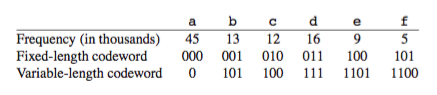
\includegraphics[scale=.7]{1.png}
\centering \linebreak \linebreak Figure 1.0: Block diagram showing part of a power supply.
\end{figure}

\subsection{IC Voltage Regulators:}

Voltage regulators comprise a class of widely used ICs. Regulator IC units contain the circuitry for reference source, comparator amplifier, control device, and overload protection all in a single IC. The IC units provide regulation of either a fixed positive voltage, a fixed negative voltage, or an adjustably set voltage. A power supply can be built using a transformer connected to the ac supply line to step the ac voltage to a desired amplitude, then rectifying that ac voltage, filtering with a capacitor and RC filter, if desired, and finally regulating the dc voltage using an IC regulator. The regulators can be selected for operation with load currents from hundreds of milliamperes to tens of amperes, corresponding to power ratings from milliwatts to tens of watts.

\subsubsection{Three-Terminal Voltage Regulator:}

\begin{multicols}{2}
Figure 1.1.1.0 shows the basic connection of a three-terminal voltage regulator IC to a load. The fixed voltage regulator has an unregulated dc input voltage, $V_{i}$, applied to one input terminal, a regulated output dc voltage, $V_{0}$, from a second terminal, with the third terminal connected to ground. For a selected regulator, IC device specifications list a voltage range over which the input voltage can vary to maintain a regulated output voltage over a range of load current. The specifications also list the amount of output voltage change resulting from a change in load current (load regulation) or in input voltage (line regulation).

\begin{figure}[H]
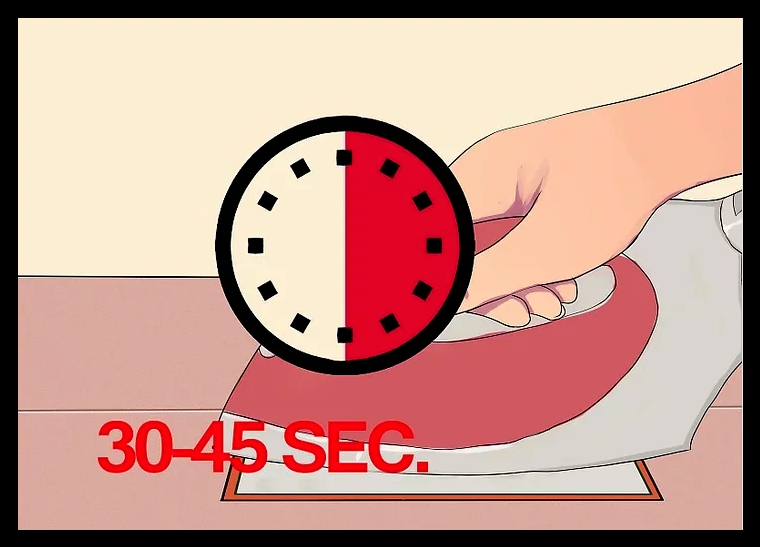
\includegraphics[scale=.45]{2.png}
\centering \linebreak \linebreak Figure 1.1.1.0: Block representation of three-terminal voltage regulator.
\end{figure}
\end{multicols}

\pagebreak

\subsubsection{Fixed Positive Voltage Regulators:}

The series 78 regulators provide fixed regulated voltages from 5 to 24 V. Figure 1.1.2.0 shows how one such IC, a {\bfseries\itshape 7812}, is connected to provide voltage regulation with output from this unit of $+$12 V dc. An unregulated input voltage $V_{i}$ it's filtered by capacitor $C_{1}$ and connected to the IC’s {\bfseries\itshape IN} terminal. The IC’s {\bfseries\itshape OUT} terminal provides a regulated $+$ 12 V, which it's filtered by capacitor $C_{2}$ (mostly for any high-frequency noise). \hfill

\begin{multicols}{2}
\begin{figure}[H]
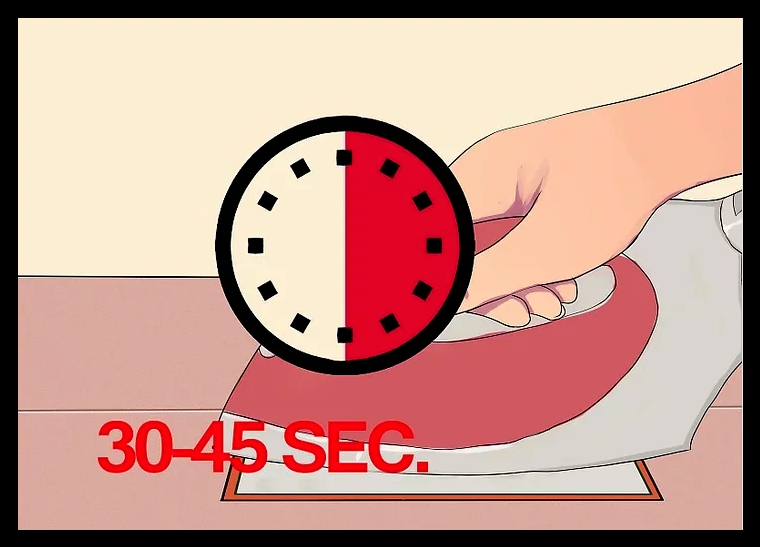
\includegraphics[scale=.45]{2.png}
\centering \linebreak \linebreak Figure 1.1.2.0: Connection of 7812 voltage regulator.
\end{figure} \hfill \break \break

The third IC terminal is connected to ground {\bfseries\itshape GND}. While the input voltage may vary over some permissible voltage range and the output load may vary over some acceptable range, the output voltage remains constant within specified voltage variation limits. These limitations are spelled out in the manufacturer's specification sheets. A table of positive voltage regulator ICs is provided in Table 1: 
\end{multicols} \hfill

\begin{multicols}{2} \hfill \break
The connection of a 7812 in a complete voltage supply is shown in the connection of Figure 1.1.2.1. The ac line voltage {\bfseries\itshape ( 120 $V_{rms}$ )} is stepped down to 18 V rms across each half of the center-tapped transformer. A full-wave rectifier and capacitor filter then provides an unregulated dc voltage, shown as a dc voltage of about 22 V, with ac ripple of a few volts as input to the voltage regulator. The 7812 IC then provides an output that is a regulated $+$ 12 V dc.

\begin{center}
{\small
\begin{tabular}[.5cm]{c c c}
\toprule
IC part & Output Voltage [ V ] & Minimum $V_{i}$ [ V ] \\
\midrule
7805 & $+$ 5 & 7.3 \\
\cmidrule{1-3}
7806 & $+$ 6 & 8.3 \\
\cmidrule{1-3}
7808 & $+$ 8 & 10.5 \\
\cmidrule{1-3}
7810 & $+$ 10 & 12.5 \\
\cmidrule{1-3}
7812 & $+$ 12 & 14.6 \\
\cmidrule{1-3}
7815 & $+$ 15 & 17.7 \\
\cmidrule{1-3}
7818 & $+$ 18 & 21.0 \\
\cmidrule{1-3}
7824 & $+$ 24 & 27.1 \\
\bottomrule
\linebreak
\end{tabular}}
\linebreak Table 1: Positive Voltage Regulators in 78xx Series.
\end{center}
\end{multicols}

\begin{figure}[H]
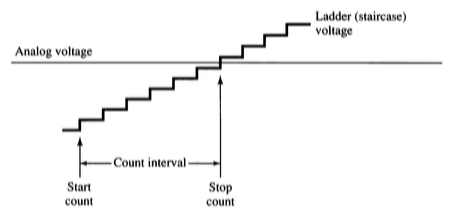
\includegraphics[scale=.6]{4.png}
\centering \linebreak \linebreak Figure 1.1.2.1:  $+$ 12 V power supply.
\end{figure}

\pagebreak

\subsubsection{Fixed Negative Voltage Regulators:}

The series 7900 ICs provide negative voltage regulators, similar to those providing positive voltages. A list of negative voltage regulator ICs is provided in Table 2. As shown, IC regulators are available for a range of fixed negative voltages, the selected IC providing the rated output voltage as long as the input voltage is maintained greater than the minimum input value. For example, the 7912 provides an output of -12 V as long as the input to the regulator IC is more negative than -14.6 V.

\begin{center}
\begin{tabular}[.5cm]{c c c}
\toprule
IC part & Output Voltage [ V ] & Minimum $V_{i}$ [ V ] \\
\midrule
7905 & $-$ 5 & -7.3 \\
\cmidrule{1-3}
7906 & $-$ 6 & -8.3 \\
\cmidrule{1-3}
7908 & $-$ 8 & -10.5 \\
\cmidrule{1-3}
7910 & $-$ 10 & -12.5 \\
\cmidrule{1-3}
7912 & $-$ 12 & -14.6 \\
\cmidrule{1-3}
7915 & $-$ 15 & -17.7 \\
\cmidrule{1-3}
7918 & $-$ 18 & -21.0 \\
\cmidrule{1-3}
7924 & $-$ 24 & -27.1 \\
\bottomrule
\linebreak
\end{tabular}
\linebreak Table 2: Negative Voltage Regulators in 79xx Series.
\end{center}

\subsubsection{Adjustable Voltage Regulators:}

Voltage regulators are also available in circuit configurations that allow the user to set the output voltage to a desired regulated value. The LM317, for example, can be operated with the output voltage regulated at any setting over the range of voltage from 1.2 to 37 V. In Figure 1.1.4.0 shows how the regulated output voltage of an LM317 can be set. \hfill \break

\begin{multicols}{2}
\begin{figure}[H]
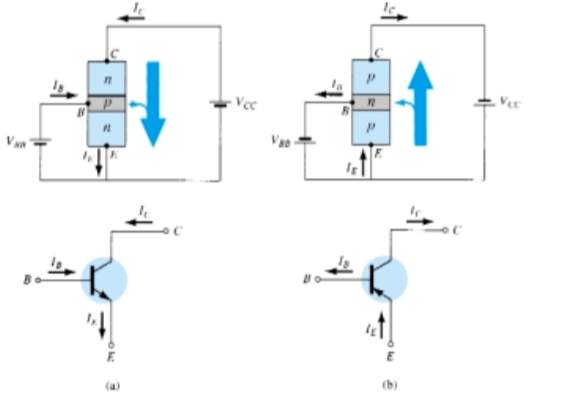
\includegraphics[scale=.6]{5.png}
\centering \linebreak \linebreak Figure 1.1.4.0: Connection of LM317 adjustable-voltage regulator.
\end{figure} \hfill \break \break \break \break

Resistors $R_{1}$ and $R_{2}$ Set the output to any desired voltage over the adjustment range (1.2 to 37 V). The output voltage desired can be calculated using: \hfill

\begin{ceqn}
\begin{align}
V_{0} = V_{ref}( 1 + \frac{R_{1}}{R_{2}} ) + I_{adj} R_{2}
\end{align}
\end{ceqn} \hfill

\end{multicols}

\pagebreak
